\chapter{Manipulation-resistant block exchange}
\label{sec:extension}
Neither a conventional blockchain solution with global consensus nor TrustChain are able fullfil all
requirements of a reporting system for encounters of a trust system. Although the scalability 
problem has been tackled by many researchers and developers\cite{poon2016bitcoin, luu2016secure}
no working solution has yet been proven in practice for blockchains with global consensus. On the 
other hand TrustChain offers a scalable solution but no strong incentive mechanism is put in place to 
ensure consistency and dissemination. 

In the previous chapter we have shown that the exchange of encounters between agents is a defense 
against inconsistent data such as forks. Also, by adding reports of exchanges to the history of 
agents, any failure to exchange will be detectable. The recording of exchanges also makes an agent's
view of the network at any given moment transparent. This can be utilized to audit any behavior in 
history of an agent.
% We claim that by 
% adding records of information exchange we are able to improve the security significantly. 
% Tamper-proof records of exchange will incentivize agents to 
% obtain and verify data. Our claims are supported by the model defined in Chapter \ref{chap:model}.

In the TrustChain architecture encounters are recorded in the form of blocks. Therefore we need to 
enable the exchange of blocks. For the implementation of block exchanges two things are required: an \textit{architecture} which enables the 
recording of exchanges and a \textit{policy} that defines which blocks to exchange and when (defined as exchange policy in 
our model). We first propose an architecture based on TrustChain which allows the implementation 
of the complete ordered encounter model from the previous chapter. The TrustChain architecture 
records an agents history on a tamper-evident chain, similar to the history of the agent in our 
model. We describe how the architecture can be extended in order to create manipulation-resistant 
evidence of block exchanges. Then we describe how the Network-State-Exchange policy can be implemented.

\begin{figure}[h!]
    \centering
    \begin{subfigure}{0.49\textwidth}
        \centering
        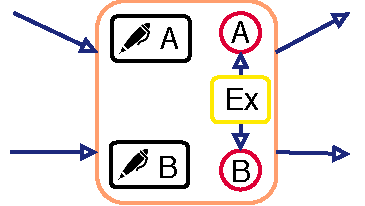
\includegraphics[width=0.8\textwidth]{images/exchange_block.pdf}
        \caption{Conceptual representation}
        \label{fig:exchange_block_conceptual}
    \end{subfigure}
    \begin{subfigure}{0.49\textwidth}
        \centering
        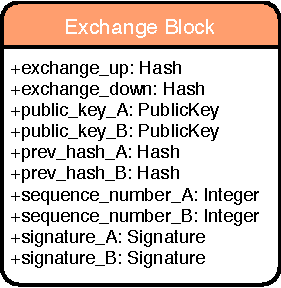
\includegraphics[width=0.6\textwidth]{images/exchange_block_data.pdf}
        \caption{Exchange block, data}
        \label{fig:exchange_block_data}
    \end{subfigure}
    \caption{A single exchange block for the TrustChain fabric. Source: \textit{Adpated from TU Delft BLockchain Lab}}
    \label{fig:exchange_block}
\end{figure}


\section{Implementation}
Exchanges can be documented in a similar way as transaction data is recorded. We extend TrustChain with \textit{exchange blocks}. Instead of the transaction
field, an exchange block contains two exchange fields which store the blocks sent and received from the perspective of
the agent that initiates the exchange. Similar to our model, an exchange consists of any type of block, so both transaction and exchange 
blocks are exchanged. 

Exchanges can become very large, in a theoretical 
worst case the whole network's data. Therefore we do not store all exchanged blocks directly but only
the root of a hash tree of the blocks. A conceptual representation and data representation 
is shown in Figure \ref{fig:exchange_block}. Note that except for the \verb|exchange_down| and \verb|exchange_up|
fields the block is similar to a transaction block as shown in Figure \ref{fig:trustchain_block}. 
The creation of the block is shown in Figure \ref{fig:block_exchange}.

Just like transaction blocks, the exchange blocks become part of an agent's chain with two incoming
and two outgoing pointers. Any exchange is recorded on-chain, creating a tamper-evident history 
of the exchange behavior provided by the TrustChain architecture.
Thus the same validity conditions apply. 


Each agent keeps track of the actual set of blocks that were received in an exchange block such that 
the root hash of the exchanged blocks can be recomputed to check the validity of the exchange block. Specifically, each 
node stores an \textit{index of the blocks} contained in an exchange in a separate database. The 
index maps an exchange block to the public key and sequence number of each
block received. This index can be 
used to retrieve the actual blocks from the database of blocks. This is illustrated in Figure \ref{fig:exchange_process}.

\begin{figure}
    \centering
    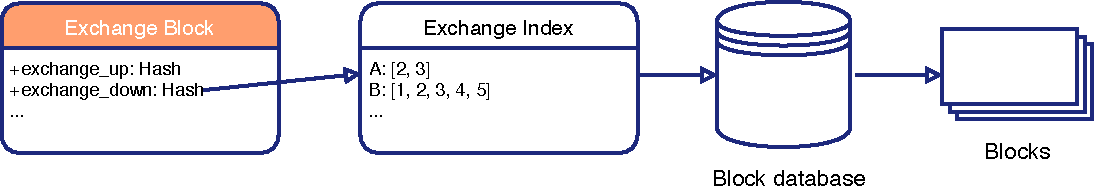
\includegraphics[width=\textwidth]{images/block_exchange_retrieval.pdf}
    \caption{Storage of exchange information: the exchange block contains a hash, which can be mapped to an index. That index can be used to retrieve the blocks from the block database.}
    \label{fig:exchange_process}
\end{figure}

With respect to our model, exchange blocks contain the agents that are involved in the exchange 
(represented by $a(e)$ in our model), whereas the root hashes of the exchanged blocks correspond to
the function $x$ in the model. Similar to $x$, the exchange hashes can only be evaluated if the 
block itself, and all exchanged blocks are available to an agent.

\begin{figure}[!ht]
    \centering
    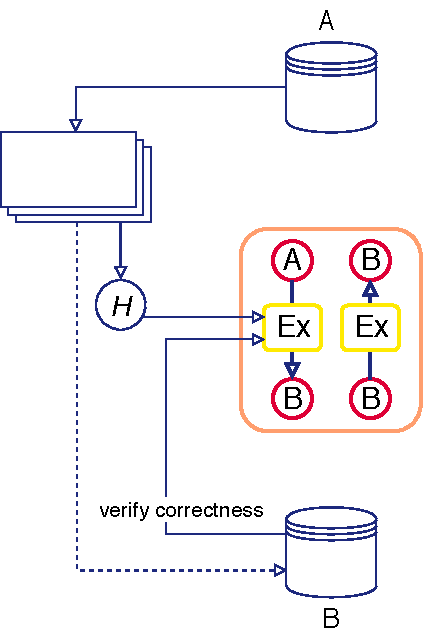
\includegraphics[width=0.4\textwidth]{images/trustchain-3.pdf}
    \caption{One half of a block exchange is shown. Agent $A$ sends blocks to $B$. $H$ creates the 
    root of a hash tree of the blocks sent. The root hash is stored in the
    exchange block. $B$ receives the blocks and can recompute the hash to verify the correctness.
    Also any other agent that has the same blocks can recompute the hash.}
    \label{fig:block_exchange}
\end{figure}

\subsection{Verification protocol}
The architecture is designed such that another node can validate the correctness of an exchange
block. Similar to the verification of transaction blocks described in Section \ref{sec:validation} an 
exchange block sequence numbers, public keys, previous hashes and signatures need to be correct. 

Additionally, the hashes stored in the \verb|exchange_down| and \verb|exchange_up| need to be valid.
An agent $A$ is able to validate an exchange between $B$ and $C$ by requesting from $B$ the blocks 
that $B$ received and from $C$ the blocks that $C$ received. If $A$ calculates the hash of $B$'s blocks
and it adds up to the hash stored in the \verb|exchange_down| and the same is true for $C$'s blocks and
the \verb|exchange_up| field, the block is valid. At this point $A$ has also established that $B$ 
and $C$ actually stored the blocks. When $A$ is only interested in confirming the honesty of one 
agent, for example $B$, $A$ can verify only the hash of the \verb|exchange_down|.

In order to validate all exchanges of one agent, the validator needs to acquire all blocks ever 
received by another agent. We showed this in Lemma \ref{lem:detection_free-rider} in Chapter \ref{chap:model}.

\subsection{Storage commitment}
An agent is committed to store the data that he received. As we have shown in this section any agent
$A$ can verify another agent $B$'s exchanges by \textit{requesting blocks}. The verification can 
only be successful if $B$ can 
summon the correct blocks. Exchanges are stored on the append-only chain where they cannot be 
removed. They can thus be verified also long after the exchange has taken place. In order to pass
verification at any time, $B$ will need to have a long-term storage for all blocks received in 
exchanges.

We define an exchange policy which requires agents to request blocks from each other. This ensures 
that block requests happen frequently and agents cannot remove any data from their database.

\subsection{Tamper-evidence and authenticity of blocks}
The tamper-evident property is inherited from the TrustChain architecture discussed in 
Section~\ref{sec:tamper-proof}. If a block is tampered with the original signatures of the block 
will be invalidated. Also any possible consecutive block's hash pointer will also be invalidated.

\section{Implementing an exchange policy}
In TrustChain the exchange behavior of agents was not visible. With the addition of exchange blocks
agents can base their decisions, for example whom to interact with, on how much data 
peers exchanged in the past. But making the gossiping behavior visible can only be the first step. 
The next step is naturally to apply the exchange records to work towards a safer distributed system.

In our model from Chapter \ref{chap:model} we defined exchange policies, which 
ensure a certain exchange of information between agents. We now consider how the
Network-State-Exchange can be implemented using the architecture defined previously. 

\subsection{Conceptual}
According to our definition an exchange policy defines a set of blocks that are required
to be exchanged prior to an interaction. Specifically, the
Network-State-Exchange policy requires two agents to exchange all blocks prior to an interactions.

This strategy combines many convenient guarantees. 
\begin{enumerate}
    \item \textit{Local consensus} is reached, such that both agents agree on a view of the network.
    \item Dissemination of all transaction blocks leads to better reputation estimates.
    \item Exchanges lead to detection of consistency issues.
    \item No agent can free-ride in storing and disseminating data because exchange behavior is 
    transparent on the chain.
    \item Collusion becomes more difficult because also any invalid blocks will be recorded in 
    exchanges creating \textit{proof-of-knowledge}.
    \item Audits of all behavior is possible. This enables \textit{guilt by association}.
\end{enumerate}

Each agent becomes a witness of their interaction partners. Through signing the exchange of all 
information they commit to storing and disseminating that information to future interaction partners.
By signing a transaction after the exchange agents commit to having verified the information of their
partner. Any fraudulent information that is ignored is recorded in the exchange block and can be 
verified in an audit as described in Chapter \ref{chap:model}.

\subsection{Completeness of exchange}
An obvious challenge of our architecture is how to ensure that agents actually act according to the
exchange policy. We claim that any honest agent is able to verify that their partner exchanged all 
information.

An honest agent $A$ exchanges blocks with $B$. $B$ sends his blocks to $A$ which includes his chain
and a block index for each exchange block on the chain. 
$A$ adds the received blocks to her database. If $A$ is now able to recalculate all exchange hashes
of the exchange blocks on $B$'s chain, using the block indexes and her own database, $A$ can be 
sure to have all blocks that $B$ has. This is similar to the evaluation of function $x$ in our model.

Note that $B$ can possible withhold blocks from the end of the chain. $A$ can only detect this if 
$A$ has received those newer blocks in some previous exchange from a third agent $C$. If $B$ withholds
blocks, $B$ is attempting to create a fork the exchange block will share a sequence number with a
block that $B$ withheld.

\subsection{Auditing}
We have shown in Chapter \ref{chap:model} that the Network-State-Exchange policy allows any honest
agent to re-evaluate any past verification of their partner. We will now describe this process, which
we call auditing. This process is the implementation of Algorithm \ref{alg:verify_exchange}.

An honest agent $A$ has exchanged blocks with $B$ and verified the completeness of their exchange.
$A$ therefore has all blocks that $B$ has. $A$ can then rebuild $B$ subjective network state, that
is the block database of the agent, at each exchange and interaction. Going through the chain of $B$, 
for each exchange block with some agent $C$, $A$ adds the blocks to the temporal subjective network
state of $B$ and checks whether $B$ was able to recalculate the exchange hashes of $C$'s exchange
blocks. Also $A$ checks whether all of $C$'s blocks are valid. For every transaction block with some
agent $D$, $A$ checks whether there was a valid exchange with $D$ prior to that transaction. Also 
$A$ checks whether $B$ was aware of any double spenders and still interacted with them afterwards. 
If that is the case $B$ is guilty by association because he is either a colluder or did not perform
verification.

If all verifications pass, $A$ has established that $B$ has throughout his complete history acted 
honestly. 

\subsection{Unresponsive agents}
Each honest agent will require an exchange with their partner prior to an interaction. If an agent 
asks a partner to send the blocks for an exchange it is possible that the partner does not respond.
This can either mean that the partner is not in the possession of the correct blocks to pass the  
verification and does not respond to not be exposed. On the other hand an agent can also be 
temporarily disconnected from the internet and therefore not able to respond. This ambiguity of not 
responding is not problematic for our solution. Any failure to respond will
lead to no further action and therefore no transaction. If however an honest agent will at some 
point respond, the verification process is continued as normal.

The situation is different if an agent stops responding in the middle of an exchange or interaction.
For example, $A$ and $B$ have exchanged data and $A$ has sent an exchange block to $B$. While waiting
for the signature of $B$, $A$ is not able to extend the chain because once $B$ eventually replies,
any extension in the meantime on $A$'s chain will create a fork. A practical solution is to create 
a timeout after which the block will be discarded. If $B$ evetually respondes, the exchange process 
needs to be repeated. 

\subsection{Efficient exchange}
Up to now we have considered that agents send all their blocks to each other. A simple efficiency 
improvement can be put in place such that only those blocks are sent which the partner does not have.

Given an agent's chain and the indexes that record which blocks were received in each exchange, any
other agent can create a complete index for the database of the other agent. That index is calculated
by combining the indexes of all exchange blocks and adding the transactions on the chain. The same
can be done for the agent himself. The difference between the two indexes are the blocks that one
agent has, but the other does not. During an exchange an agent can then specifically request only
those blocks. Therefore exchanges become a synchronization in which differences between the states
are resolved. Note that if both agents have different blocks of a double spend such, that block will
not be synchronized with this method. However, the difference will be detected when controlling the
hash.

\begin{figure}[!ht]
    \centering
    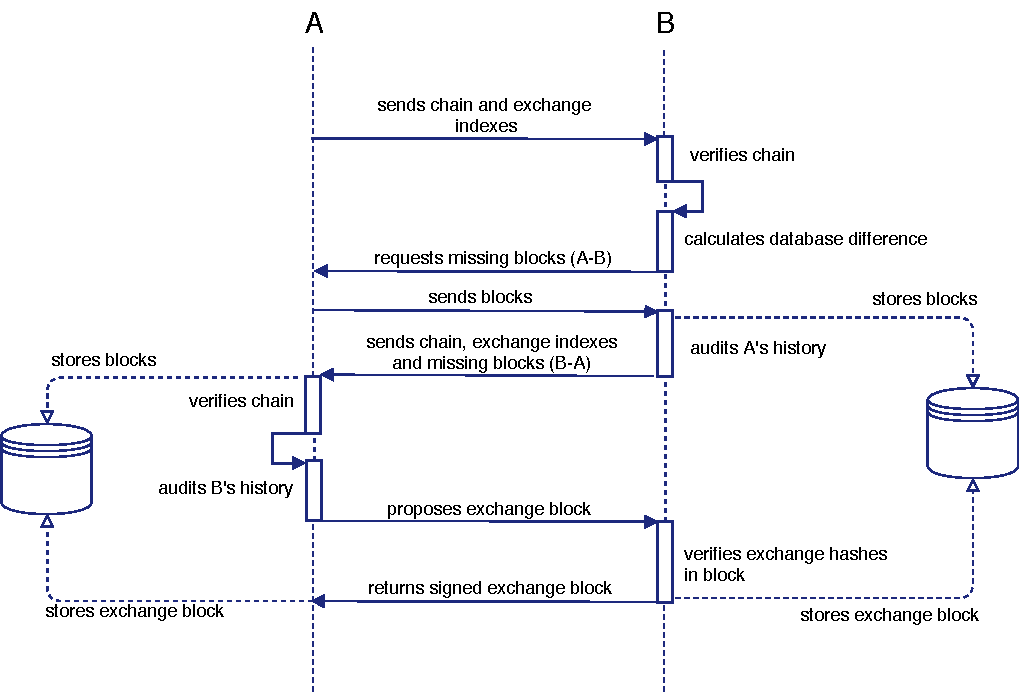
\includegraphics[width=\textwidth]{images/exchange_process.pdf}
    \caption{Exchange process between two agents $A$ and $B$.}
    \label{ref:exchange_process}
\end{figure}

\subsection{Exchange process}
We shall now describe the complete process of an exchange between two agents in detail. The process
is also shown in Figure \ref{ref:exchange_process}. Thus, $A$ 
initiates the exchange by sending $A$'s complete chain to $B$, together with a block index for each 
exchange block.
$B$ can perform simple checks on the chain, for example whether it contains the correct number of exchange blocks
according to the exchange policy and whether all blocks are correctly signed and chained. From the 
chain and the exchange block indexes, $B$ is able to reconstruct the complete database index of $A$.

Given $A$'s database index, $B$ can calculate the difference between their databases. $B$ will 
then request from $A$ the blocks that $A$ has but $B$ does not. Once $A$ replies, $B$ has all 
information that $A$ has. $A$'s subjective network state has become transparent to $B$. 

$B$ is then able to perform the audit of $A$. If $A$'s behavior as recorded by the chain is correct, 
$B$ sends his chain, exchange
indexes and blocks to $A$. Note that $B$ already knows which blocks $A$ is missing with respect to 
$B$ and can therefore directly send them. 

Now $A$ is able to perform the same checks as $B$. If $B$'s data also checks out, $A$ will create 
a new exchange block. The exchange block contains the root hash of the blocks that $A$ uploaded to $B$ 
and downloaded from $B$. As $B$ also knows which blocks he received from $A$ and sent to $A$, $B$ should
be able to calculate the same hashes. After both parties sign the block, they add them to their 
database of blocks. Also they create an entry for the exchange block in the exchange index map, which 
maps each exchange block to the index of exchanged blocks. At this point they have concluded the 
exchange according to the Network-State-Exchange policy.

\subsection{Consistency and Scalability consideration}
For each interaction the Network-State-Exchange policy requires a node $A$ to obtain all the blocks that
their partner $B$ is aware of. If that $B$ is honest, this includes also all the knowledge of all of
$B$'s peers. Consequently each agent will approximate the full network state. This requires the 
storage of all blocks on the network. 

The process is similar to the anti-entropy mechanism defined 
in Demers et al. \cite{demers1987epidemic}. If we assume agents randomly chose their next interaction
partner the two mechanisms are similar. Therefore a similar performance can be expected. Anti-entropy,
being an epidemic algorithm, will eventually distribute updates to all nodes in an expected time 
proportional to the log of the population size.

The mechanism therefore disseminates updates to all nodes which leads to consistency and enables 
indirect reciprocity because all agents can have a good estimate of each others reputation and trust.

On the downside this mechanism will not scale. Although each exchange and 
transaction still only requires two agents to communicate as in the example given in 
Section \ref{sec:trustchain_scalability} storing all data is not an option if proper global throughput
is required. In Section \ref{sec:system_trust} we explore different exchange policies that might 
allow better scalability at lower storage cost.

\section{Example}
We now consider an example to shed more light of the exchange and interaction process. We look at two
agents, Alice and Bob. Alice wants to interact with Bob and starts the interaction. We assume that
both agents are new to the network and only have their genesis blocks on the chain. In order to
start the interaction, Alice sends her chain (only the genesis block) and an empty set of exchanges
to Bob. Obviously the genesis block is accepted and Bob shows his approval by sending his own
genesis block and an empty set of exchanges. Also Alice accepts the data. 

Alice creates an exchange
block which includes in the field \verb|exchange_up| the hash of Alice's genesis block and in the field 
\verb|exchange_down| the hash of Bob's genesis block. Alice signs that block and sends it to Bob. 
Bob verifies that the hashes actually are correct. If Bob agrees, he also signs the block and returns 
it to Alice. Both Bob and Alice now store the block with both signatures in their database of blocks.
Alice also stores a block index for the created exchange block which includes as entry 
only Bob's block with sequence number 1. Similarly, Bob documents that he received Alice's first block
in the new exchange block.

At this point both agents are sure that they are honest and are able to interact in the 
application context. For example, Alice could now stream a video from Bob in Tribler. After the transaction in 
the application context, Alice creates and signs a transaction block and sends it to Bob who replies 
in a similar fashion if he agrees. Figure \ref{fig:exchange_example} shows the chains of Alice and 
Bob after the complete interaction. 

\begin{figure}
    \centering
    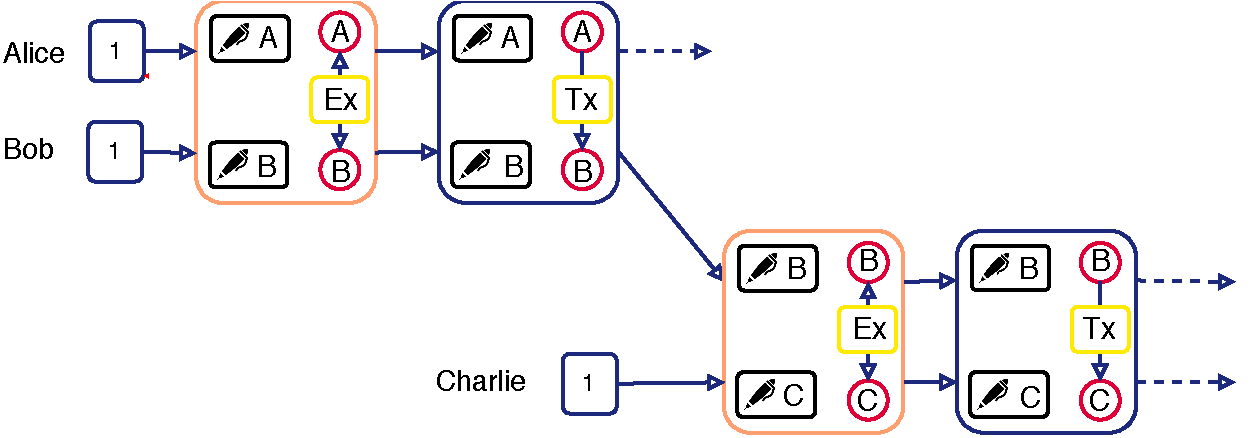
\includegraphics[width=\textwidth]{images/trustchain_example.pdf}
    \caption{Example of three agents interacting}
    \label{fig:exchange_example}
\end{figure}

This example sheds light on the block creation process but is too simple to properly explain the 
exchange and verification process. We extend the example with another agent, Charlie, whom Bob would
like to interact with after the previous interactions. Again, Charlie is assumed to be new to the 
network so the genesis block is the only block on his chain. Bob starts the interactions by sending
his chain and the index that documents the acquisition of Alice's first block. 

Charlie sees that Bob has an exchange block with Alice before have a transaction with her, which is 
correct according to the exchange policy. Next Charlie checks the signatures and hashes of Bob's chain. 
After those checks pass, Charlie tries to calculate the hashes for Bob's exchange block but realizes
that he does not have Alice's first block. Therefore he requests it from Bob. After receiving it the
check should pass. 

Once Charlie accepts all the checks, he sends his own chain and exchanges which are checked by Bob
and the interaction continues as previously described. Table \ref{tab:blocks_example} shows the
blocks that each agent has after the first and second round. After the second round, Charlie has 
all the blocks from Bob that he had after the first round.

\begin{table}[h!]
    \centering
    \caption{The block databases of each agent for the example}
    \label{tab:blocks_example}
    \begin{tabular}{p{4cm}|p{3cm}|p{4cm}|p{3cm}}
        \toprule
        Database & Alice & Bob & Charlie \\
        \midrule
        Before first round & A: $[1]$ & B: $[1]$ & C: $[1]$ \\ \hline 
        After first round & A: $[1, 2, 3]$ \newline B: $[1, 2, 3]$ & A: $[1, 2, 3]$ \newline B: $[1, 2, 3]$ & C: $[1]$ \\ \hline
        After second round &  A: $[1, 2, 3]$ \newline B: $[1, 2, 3]$ & A: $[1, 2, 3]$ \newline B: $[1, 2, 3, 4, 5]$ \newline C: $[1, 2, 3]$ & A: $[1, 2, 3]$ \newline B: $[1, 2, 3, 4, 5]$ \newline C: $[1, 2, 3]$ \\
        \bottomrule
    \end{tabular}
\end{table}


% \subsection{Obtaining a subject network state}
% One property of the extended architecture that we proposed in this section is that an agent's complete
% database is transparent to other nodes. It enables nodes to explore another node's view of the network. 
% In our model we called this the subjective network state. 

% Specifically, a node $A$ obtains a complete
% chain from an agent $B$ which includes transaction and exchange blocks. Furthermore, for each exchange 
% $B$ provides $A$ with the index of blocks contained in that exchange. If $A$ is able to recalculate 
% all the exchange hashes stored in the exchange blocks of $B$, $A$ has at least all information that 
% $B$ has and is able to obtain an exact similar subjective network state as $B$. If not, $A$ can see 
% from the exchange indexes which blocks $B$ has that $A$ does not. $A$ can request those from $B$, and
% if $B$ is honest $B$ will respond. Finally, 


% Exchange policies allow the system designer to ship software with a less or more stringent
% exchange policy. This will reduce or increase security but also impact the requirements on storage and bandwidth.
% If a stringent policy is applied, it should be possible to delete data. This could also be recorded on chain. As only the 
% root hash of the exchanges are stored on an agents chain, a delete block should be possible by 
% recording in a similar fashion without the need to remove blocks from the chain. Therefore chain 
% consistency is kept intact. How this should be implemented in detail and a security analysis will 
% be left for future research.

\section{Other exchange policies}
\label{sec:system_trust}
The architecture that we have presented in the previous section is very flexible. Any size of information 
exchange between two parties can be recorded. It therefore allows for the implementation of any 
exchange policy. We described in the previous section how the Network-State-Exchange policy can be implemented
and that it can give strong guarantees for security but also induces the highest cost on storage and bandwidth 
capacity. Depending on the application this might be necessary however TrustChain was designed to 
be as scalable as possible without global consensus. Therefore also less demanding exchange policies
can be implemented.

In our model we describe the exchange-history policy. We show that it is enough to detect forks 
and honest agents can still ensure that their exchanges are correct. However, no previous exchanges 
can be verified as with the audit protocol. This policy therefore trades some consistency and 
correctness guarantees for less storage and bandwidth requirements. Similarly other policies can 
be explored.

Instead of enforcing a certain policy, the exchange records can also be used to create a system level 
notion of trust. Instead of verifying every agent before every interaction, each successful verification
of an agent can lead to trust between the two. This would create a reputation system based on the
adherence to the system-level requirements of good behavior. 


% \section{Attacks}
% We now consider possible ways to attack the 

% \subsection{Block tampering}
% Similar to the block tampering that we described in Section \ref{sec:tampering}, an agent could 
% directly change the hash of received blocks after an exchange. Again, the signature of the partner 
% stored in the block will be invalidated. 

% \subsection{Not actually storing information}
% The information that is received is only recorded in form of the root hash of contained blocks. The 
% actual blocks are in the database of the agent itself which is obviously opaque to other agents. 
% Therefore an agent $A$ could possible only record correctly the exchange but not actually store the 
% received information. 

% However, other agents are expecting $A$ to be in the possession of the block. Thus, depending 
% on the exchange policy, an agent might at some point request a block in which case $A$ is not able 
% to respond. This will expose the agent of free-riding on the storage.

% \paragraph{Collusion}
% As we have previously discussed in Section \ref{sec:collusion}, attacking agents can work together in 
% a collusion attack. We claim that a subset of those collusion attacks is more difficult if agents are
% able to obtain subjective network state transparency. Consider two agents $A$ and $B$ are colluding 
% in a block tampering. $B$ has changed a block in order to obtain more reputation and $A$ is transacting 
% with $B$ to receive some of the maliciously gained reputation. But in order to transact and be considered
% an honest agent, $B$ needs to obtain $A$'s chain. In that case 

% * Verification and exchanges make an agent trustworthy on a system level, as in, we trust them to 
% stick to the rules of recording, exchanging and verifying
% * Use this to not verify each and every agent, but assume agent which were verified by trustworthy
% agents to be trustworthy enough for interaction
% * At every point we still have the chance to do the complete verification of a history. But maybe 
% its not required every turn

\section{Chapter conclusion}
We have defined an extension to the original TrustChain architecture which allows for the exchange 
of blocks. We have shown how this architecture can be used to exchange data and enforce an 
exchange policy. Also, we have defined an audit protocol which allows for the complete verification
of agents data. 

The exchange policy ensure that data is disseminated while a strong policy like the Network-State-Exchange
policy allow for strong consistency guarantees. We have theoretically established this in the 
previous chapter as well. Therefore this architecture is very much useful for a trust system as we
envision it. On the other hand, scalability will become an issue as verification will become more
elaborate with increasing chain lengths and storage requirements grow. 

An alternative to enforcing an exchange policy can be to define a system-level trust system such that
verifications can happen less frequently and verified partner become trusted peers. This way agents
can interact with any other verified partners of their trusted peers without redoing the verification.
We consider this a possibility for future research.